
\documentclass{beamer}
\usecolortheme{dove}
\setbeamertemplate{navigation symbols}{}
\usepackage{amsmath,amssymb,amsfonts,amsthm, multicol, subfigure, color}
\usepackage{bm}
\usepackage{graphicx}
\usepackage{tabularx}
\usepackage{booktabs}
\usepackage{hyperref}
\usepackage{pdfpages}
\usepackage{xcolor}
\definecolor{seagreen}{RGB}{46, 139, 87}
\def\independenT#1#2{\mathrel{\rlap{$#1#2$}\mkern2mu{#1#2}}}
\newcommand\indep{\protect\mathpalette{\protect\independenT}{\perp}}
\def\log{\text{log}}
\newcommand\logit{\text{logit}}
\newcommand\iid{\stackrel{\text{iid}}{\sim}}
\newcommand\E{\text{E}}
\newcommand\V{\text{V}}
\renewcommand\P{\text{P}}
\newcommand{\Cov}{\text{Cov}}
\newcommand{\Cor}{\text{Cor}}
\newcommand\doop{\texttt{do}}
\usepackage{stackrel}
\usepackage{tikz}
\usetikzlibrary{arrows,shapes.arrows,positioning,shapes,patterns,calc}
\newcommand\slideref[1]{\vskip .1cm \tiny \textcolor{gray}{{#1}}}
\newcommand\red[1]{\color{red}#1}
\newcommand\blue[1]{\color{blue}#1}
\newcommand\gray[1]{\color{gray}#1}
\newcommand\seagreen[1]{\color{seagreen}#1}
\newcommand\purple[1]{\color{purple}#1}
\newcommand\orange[1]{\color{orange}#1}
\newcommand\black[1]{\color{black}#1}
\newcommand\white[1]{\color{white}#1}
\newcommand\teal[1]{\color{teal}#1}
\newcommand\magenta[1]{\color{magenta}#1}
\newcommand\Fuchsia[1]{\color{Fuchsia}#1}
\newcommand\BlueGreen[1]{\color{BlueGreen}#1}
\newcommand\bblue[1]{\textcolor{blue}{\textbf{#1}}}
\newcommand\bred[1]{\textcolor{red}{\textbf{#1}}}
\newcommand\bgray[1]{\textcolor{gray}{\textbf{#1}}}
\newcommand\bgreen[1]{\textcolor{seagreen}{\textbf{#1}}}
\newcommand\bref[2]{\href{#1}{\color{blue}{#2}}}
\colorlet{lightgray}{gray!40}
\pgfdeclarelayer{bg}    % declare background layer for tikz
\pgfsetlayers{bg,main} % order layers for tikz
\newcommand\mycite[1]{\begin{scriptsize}\textcolor{darkgray}{(#1)}\end{scriptsize}}
\newcommand{\tcframe}{\frame{
%\small{
\only<1|handout:0>{\tableofcontents}
\only<2|handout:1>{\tableofcontents[currentsection]}}
%}
}

\usepackage[round]{natbib}
\bibliographystyle{humannat-mod}
\setbeamertemplate{enumerate items}[default]
\usepackage{mathtools}

\newcommand{\goalsframe}{\begin{frame}{Learning goals for today}
At the end of class, you will be able to:
\begin{enumerate}
\item Use machine learning methods to estimate causal effects
\item Select an estimator using predictive performance
\end{enumerate} \vskip .2in
\end{frame}}

\title{10. The generality of the g-formula: Using any estimator}
\author{Ian Lundberg\\Cornell Info 6751: Causal Inference in Observational Settings\\Fall 2022}
\date{22 Sep 2022}

\begin{document}

\maketitle

\goalsframe

\begin{frame}{You are now well-versed in the g-formula}

\begin{enumerate}
\item Assume a DAG
\begin{center}
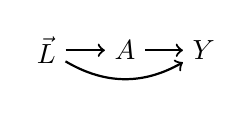
\begin{tikzpicture}
\node (l) at (-1,0) {$\vec{L}$};
\node (a) at (0,0) {$A$};
\node (y) at (1,0) {$Y$};
\draw[->, thick] (l) -- (a);
\draw[->, thick] (l) to[bend right] (y);
\draw[->, thick] (a) -- (y);
\end{tikzpicture}
\end{center}
\item By consistency, exchangeability, and positivity, $$\underbrace{\E(Y^a\mid\vec{L} = \vec\ell)}_{\text{Causal}} = \underbrace{\E(Y\mid A = a, \vec{L} = \vec\ell)}_{\text{Statistical}}$$
\item Using regression, estimate $\hat\E(Y\mid A, \vec{L})$
\item Predict unknown potential outcomes and average
$$\hat\E(Y^a) = \frac{1}{n}\sum_{i=1}^n \hat\E\left(Y\mid A = a, \vec{L} = \vec\ell_i\right)$$
\end{enumerate}
\bblue{Big idea:} Why constrain ourselves to regression for $\hat\E(Y\mid A, \vec{L})$?

\end{frame}

\begin{frame}

Hill, Jennifer L. 2011.\\``\bref{https://doi.org/10.1198/jcgs.2010.08162}{Bayesian nonparametric modeling for causal inference.}"\\Journal of Computational and Graphical Statistics 20.1:217-240. \vskip .1in
\begin{itemize}
\item Binary treatment \hfill (simulated)
\item Continuous confounder $X$ \hfill (simulated)
\end{itemize} \vskip .1in
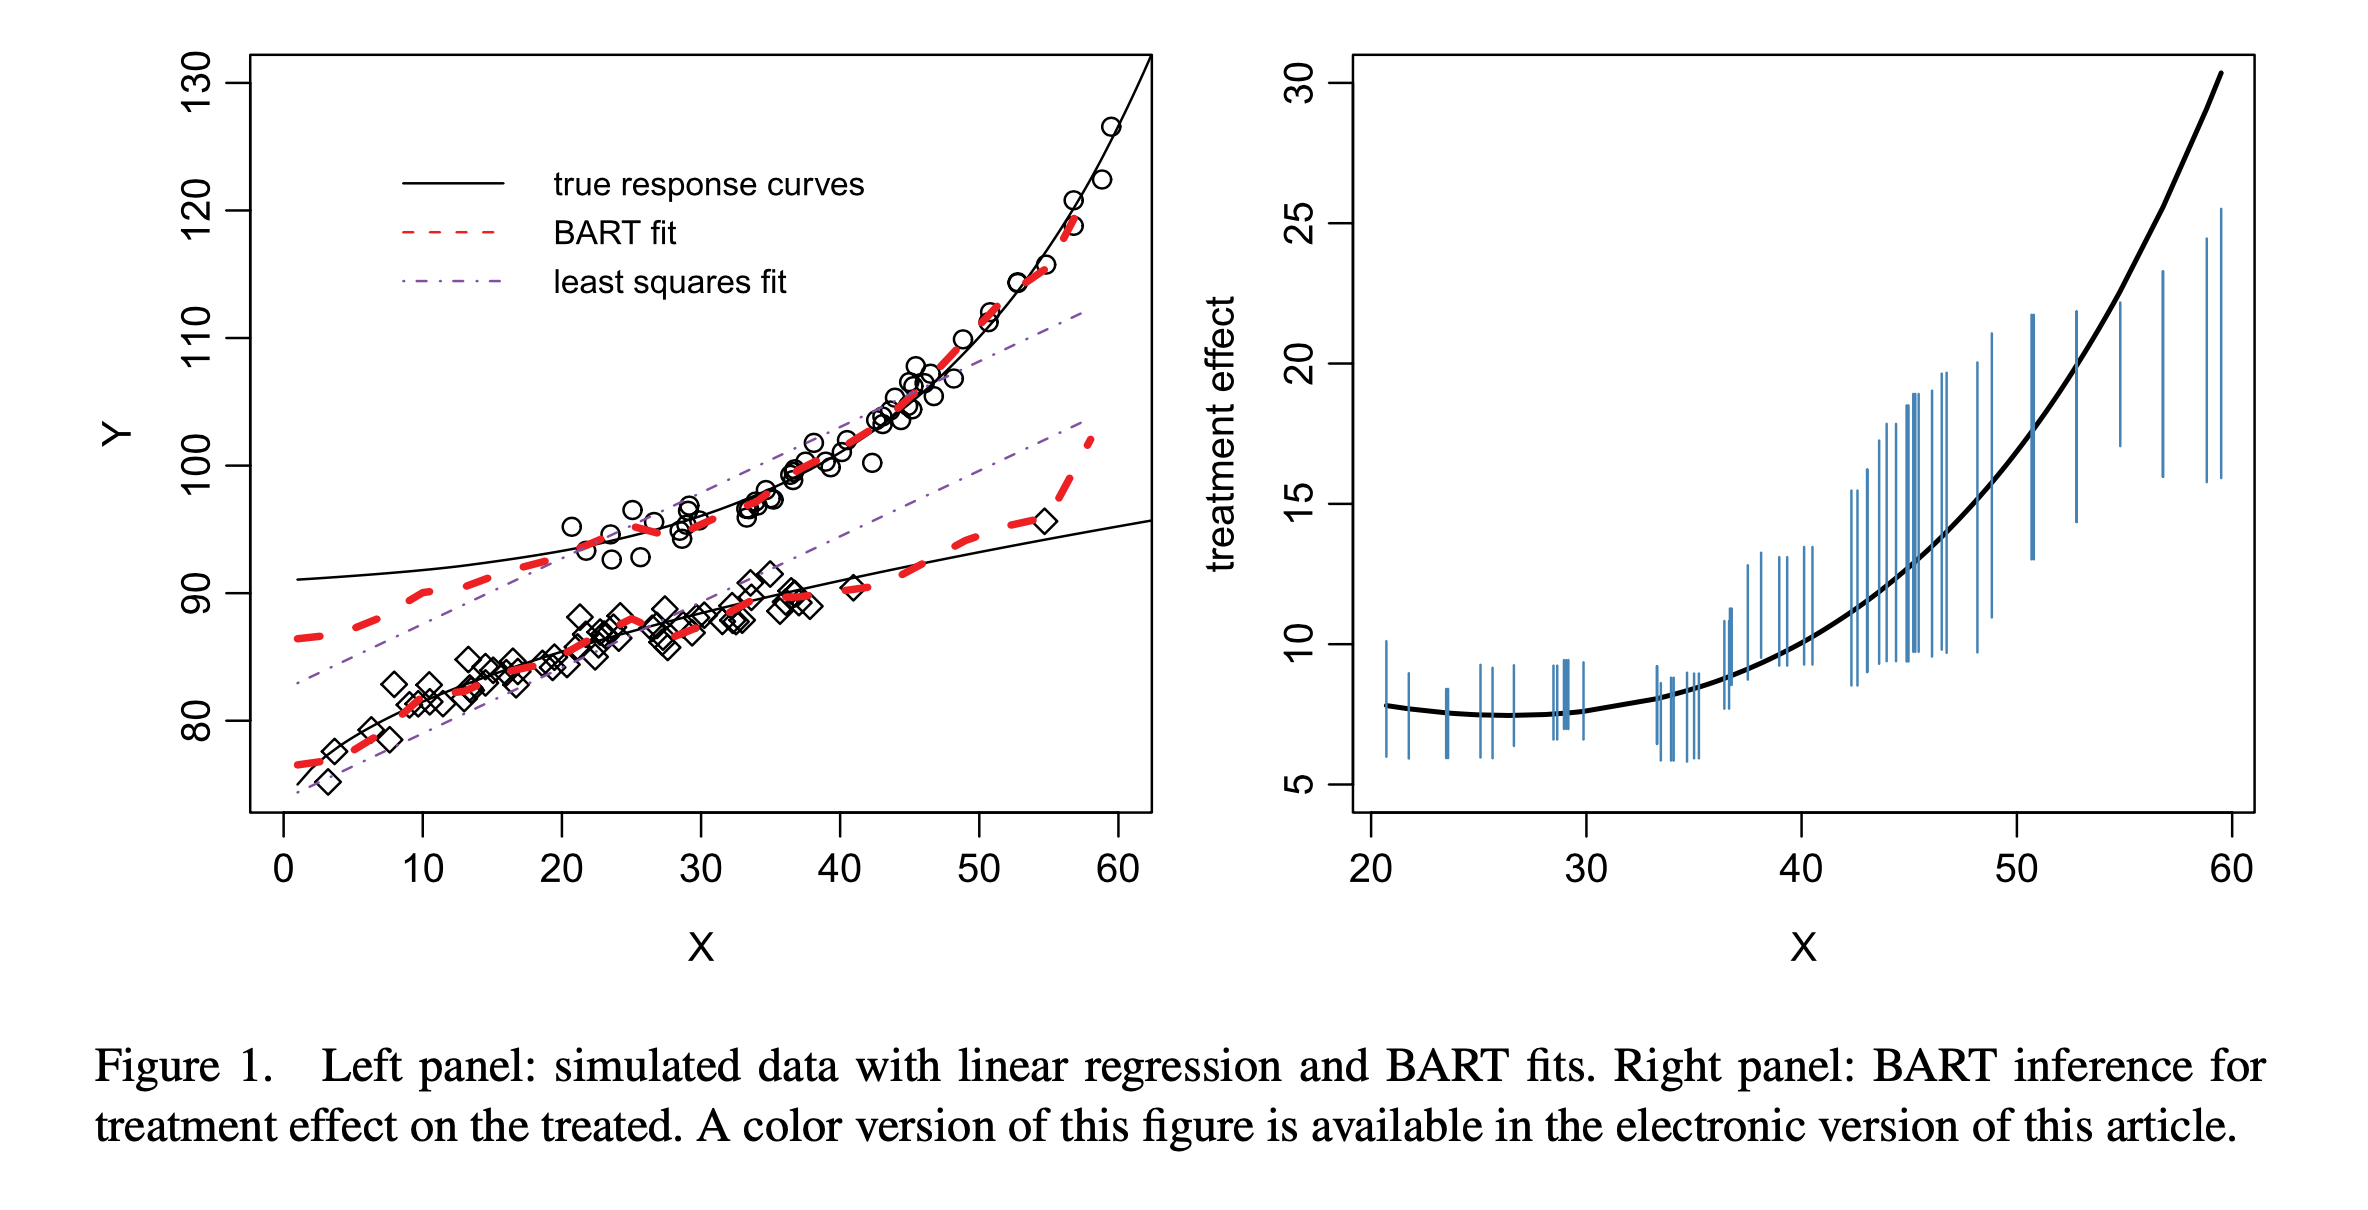
\includegraphics[width = \textwidth]{figures/hill2011_fig1}

\end{frame}

\begin{frame}[t]{How did she do that?\footnote{Chipman, Hugh A., Edward I. George, and Robert E. McCulloch. ``\bref{https://projecteuclid.org/journals/annals-of-applied-statistics/volume-4/issue-1/BART-Bayesian-additive-regression-trees/10.1214/09-AOAS285.full}{BART: Bayesian additive regression trees.}" The Annals of Applied Statistics 4.1 (2010): 266-298.}}
\vskip .2in
1) Learn an automated partitioning of the data (aka a ``tree'')
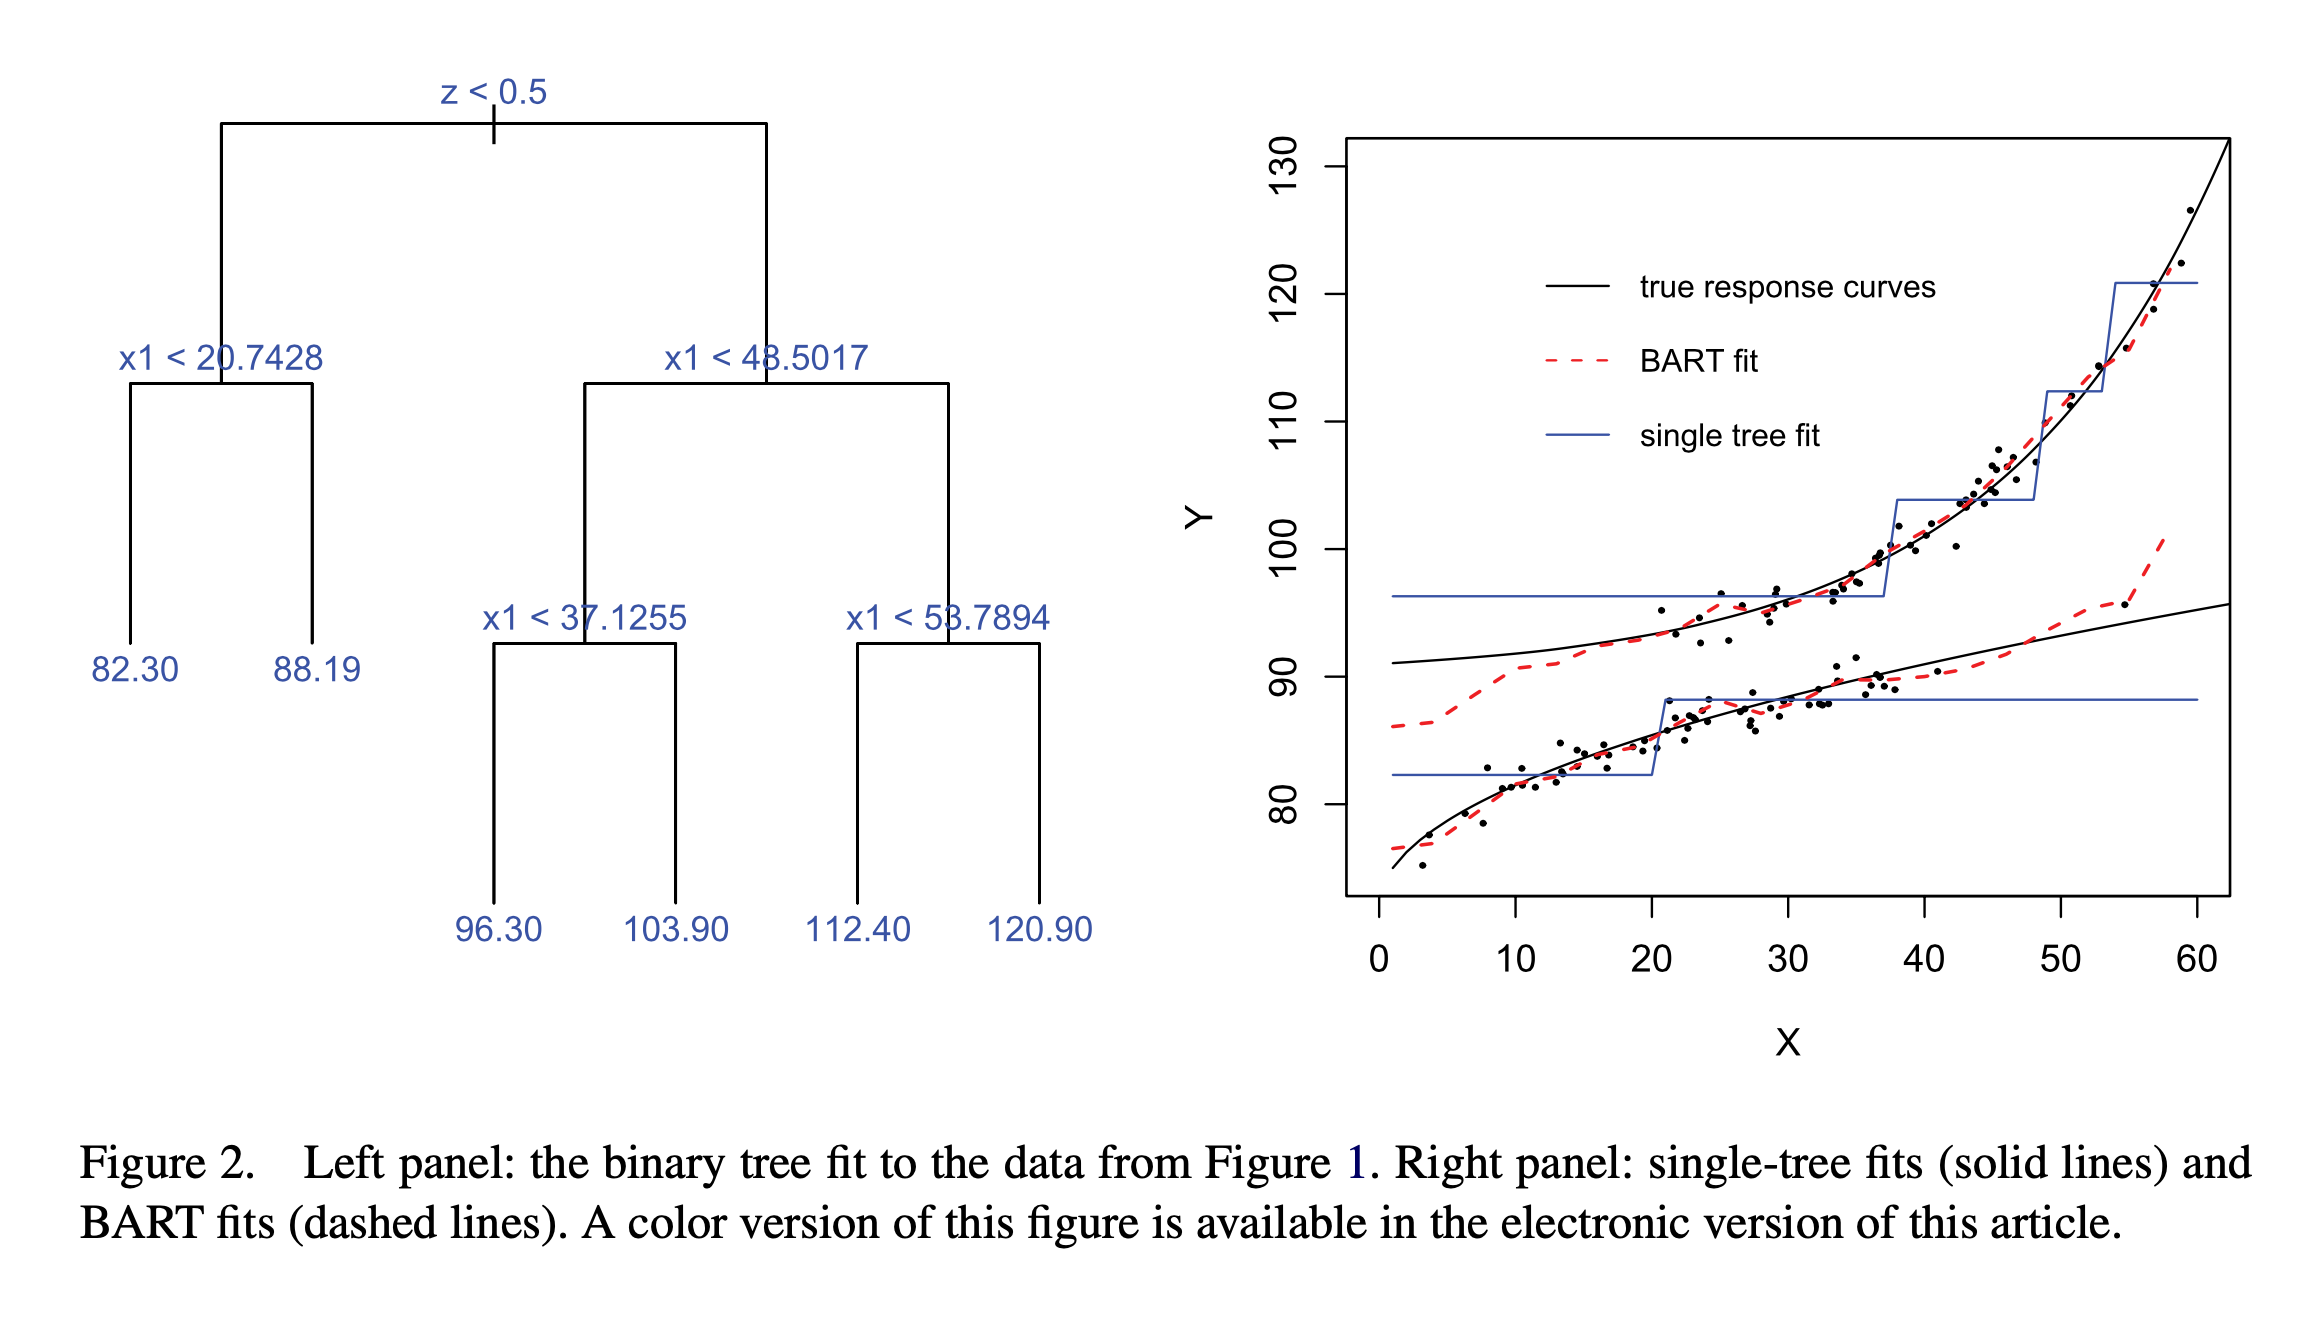
\includegraphics[width = \textwidth]{figures/hill2011_fig2}
\end{frame}

\begin{frame}[t]{How did she do that?}
\vskip .2in
2) Repeat many times. Take the average.\\
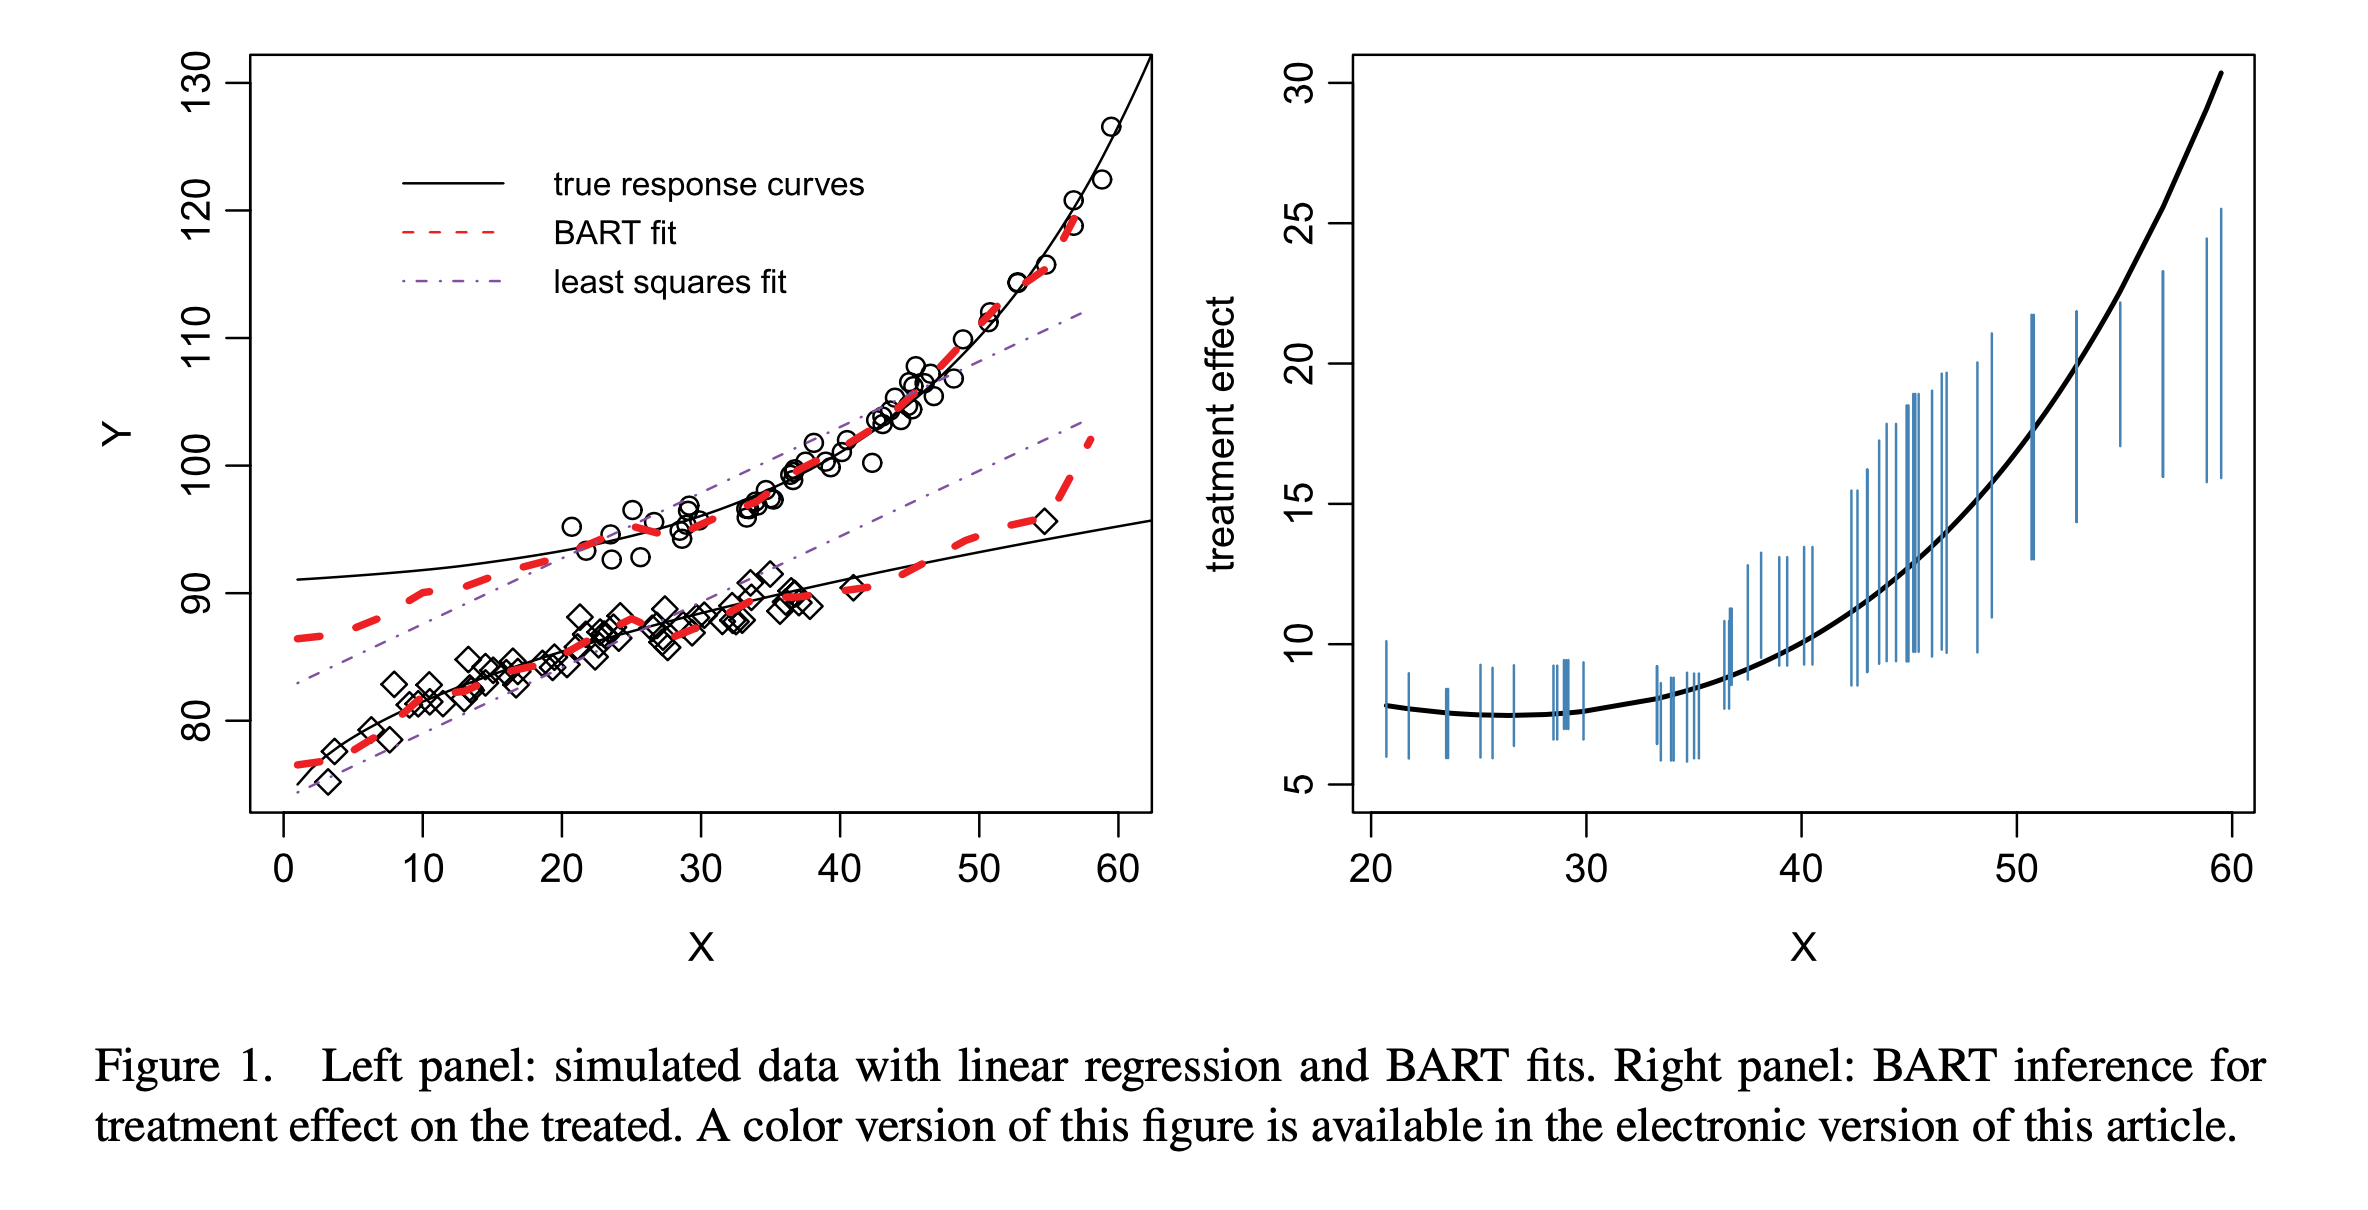
\includegraphics[width = \textwidth]{figures/hill2011_fig1}
\end{frame}

\begin{frame}{Core idea: Causal assumptions unlock machine learning\footnote{Caveat: There are ways to do even better. This is just a start.\\See Van der Laan, M. J., \& Rose, S. (2018). \bref{https://link.springer.com/content/pdf/10.1007/978-3-319-65304-4.pdf}{Targeted learning in data science.} Springer International Publishing.}}
Once you make this assumption
\begin{center}
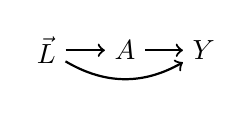
\begin{tikzpicture}
\node (l) at (-1,0) {$\vec{L}$};
\node (a) at (0,0) {$A$};
\node (y) at (1,0) {$Y$};
\draw[->, thick] (l) -- (a);
\draw[->, thick] (l) to[bend right] (y);
\draw[->, thick] (a) -- (y);
\end{tikzpicture}
\end{center}
you get to do this
\begin{center}
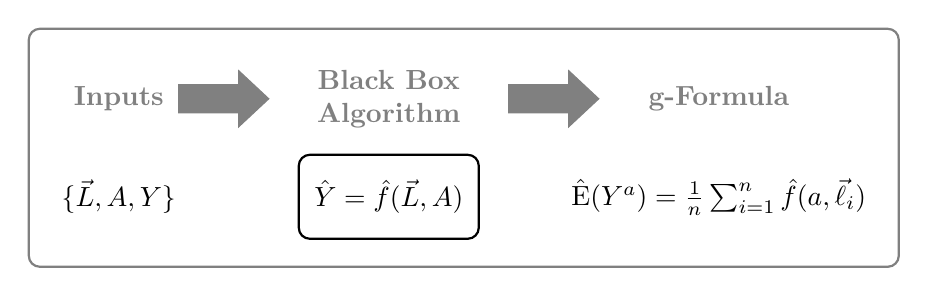
\begin{tikzpicture}[x = 1.5in, y = .7in]
\node[gray, font = \bf] at (-1,.7) {Inputs};
\node[align = center, gray, font = \bf] at (-.1,.7) {Black Box\\Algorithm};
\node[gray, font = \bf] at (1,.7) {g-Formula};
\node at (-1,0) {$\{\vec{L},A,Y\}$};
\node at (-.1,0) {$\hat{Y} = \hat{f}(\vec{L},A)$};
\node at (1,0) {$\hat\E(Y^a) = \frac{1}{n}\sum_{i=1}^n \hat{f}(a,\vec\ell_i)$};
\draw[thick, rounded corners] (-.4,-.3) rectangle (.2,.3);
\draw[thick, gray, rounded corners] (-1.3,-.5) rectangle (1.6, 1.2);
\draw[draw = gray, fill = gray] (-.8,.8) -- (-.8,.6) -- (-.6,.6) -- (-.6,.5) -- (-.5,.7) -- (-.6,.9) -- (-.6,.8) -- cycle;
\draw[draw = gray, fill = gray] (.3,.8) -- (.3,.6) -- (.5,.6) -- (.5,.5) -- (.6,.7) -- (.5,.9) -- (.5,.8) -- cycle;
\end{tikzpicture}
\end{center}
\end{frame}

\begin{frame}
There are \bblue{so many} algorithms you might use!
\end{frame}

\begin{frame}
\centering
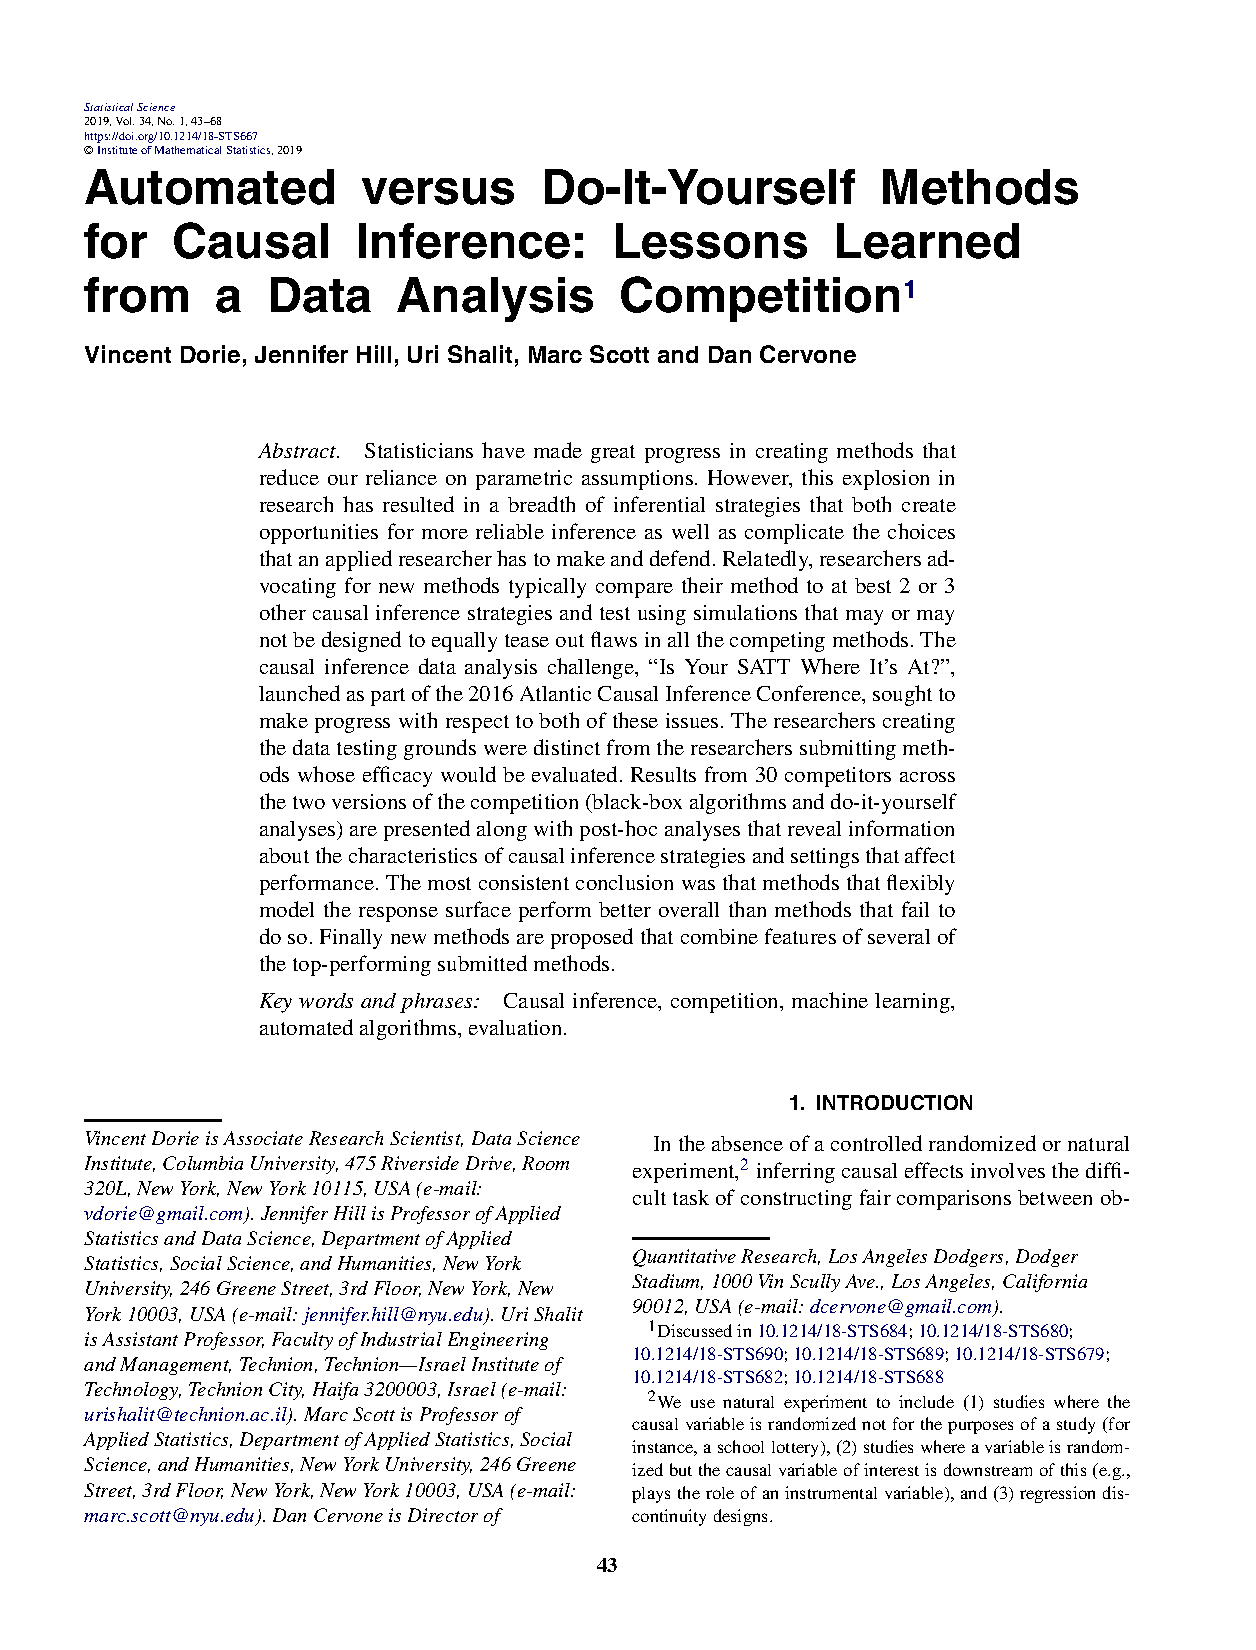
\includegraphics[height = \textheight]{figures/dorie_p1}
\end{frame}

\begin{frame}{Dorie et al. 2019\footnote{
Dorie, V., Hill, J., Shalit, U., Scott, M., \& Cervone, D. (2019).\\
``\bref{https://projecteuclid.org/journals/statistical-science/volume-34/issue-1/Automated-versus-Do-It-Yourself-Methods-for-Causal-Inference/10.1214/18-STS667.full}{Automated versus do-it-yourself methods for causal inference: Lessons learned from a data analysis competition.}'' Statistical Science, 34(1), 43-68. See also \blue{\url{https://jenniferhill7.wixsite.com/acic-2016/competition}}}: Is Your SATT Where It's At?}

\begin{itemize} \pause
\item Goal: The Sample Average Treatment Effect on the Treated
$$\text{SATT} = \frac{1}{n_\text{Treated}}\sum_{i:A_i = 1} \left(Y_i^1 - Y_i^0\right)$$ \pause
\item Simulated data. SATT was known to organizers \pause
\item Confounders were defined by the organizers \pause
\item Participants could use any algorithm to estimate SATT \pause
\item 30 teams attempted the task \pause
\item Today you will attempt it!
\end{itemize}

\end{frame}

\begin{frame}{A few things to help you succeed}
\begin{enumerate}
\item A few algorithms you might consider
\begin{itemize}
\item Ridge, LASSO, elastic net \hfill (\texttt{glmnet})
\item Random forest \hfill (\texttt{ranger})
\item Bayesian additive regression trees \hfill (\texttt{BART})
\item Super Learner \hfill (\texttt{SuperLearner})
\end{itemize}
\item How do I choose a black-box algorithm?
\item Overview of the data structure
\end{enumerate}
\end{frame}

\begin{frame}{A few algorithms you might consider: \texttt{glmnet}}
\begin{itemize}
\item Idea: With many coefficients, OLS can by high-variance.
\item \texttt{glmnet} \bblue{penalizes} coefficients to reduce sample variance
\begin{itemize}
\item Pushes coefficeints toward 0
\item When we are uncertain about $\hat\beta$, better to keep $\hat\beta$ small
\end{itemize}
\item Three ways to penalize
\begin{itemize}
\item Ridge penalty: Minimize $\frac{1}{n}\sum_{i=1}^n (\hat{Y}_i - Y_i)^2 + \lambda\sum_j \beta_j^2$
\begin{itemize}
\item Coefficients are pulled toward 0, but not exactly to 0
\end{itemize}
\item Lasso penalty: Minimize $\frac{1}{n}\sum_{i=1}^n (\hat{Y}_i - Y_i)^2 + \lambda\sum_j \lvert \beta_j\rvert$
\begin{itemize}
\item Some coefficients pushed exactly to 0 (dropped out entirely)
\end{itemize}
\item Elastic net: Penalize both $\beta_j^2$ and $\lvert \beta_j\rvert$
\end{itemize}
\end{itemize}
\end{frame}

\begin{frame}{A few algorithms you might consider: \texttt{ranger}\footnote{Wright, M. N., \& Ziegler, A. (2017). \bref{http://dx.doi.org/10.18637/jss.v077.i01}{ranger: A fast implementation of random forests for high dimensional data in C++ and R.} Journal of Statistical Software, 77(i01).}}
\begin{itemize}
\item Random forest: A frequentist sum-of-trees model
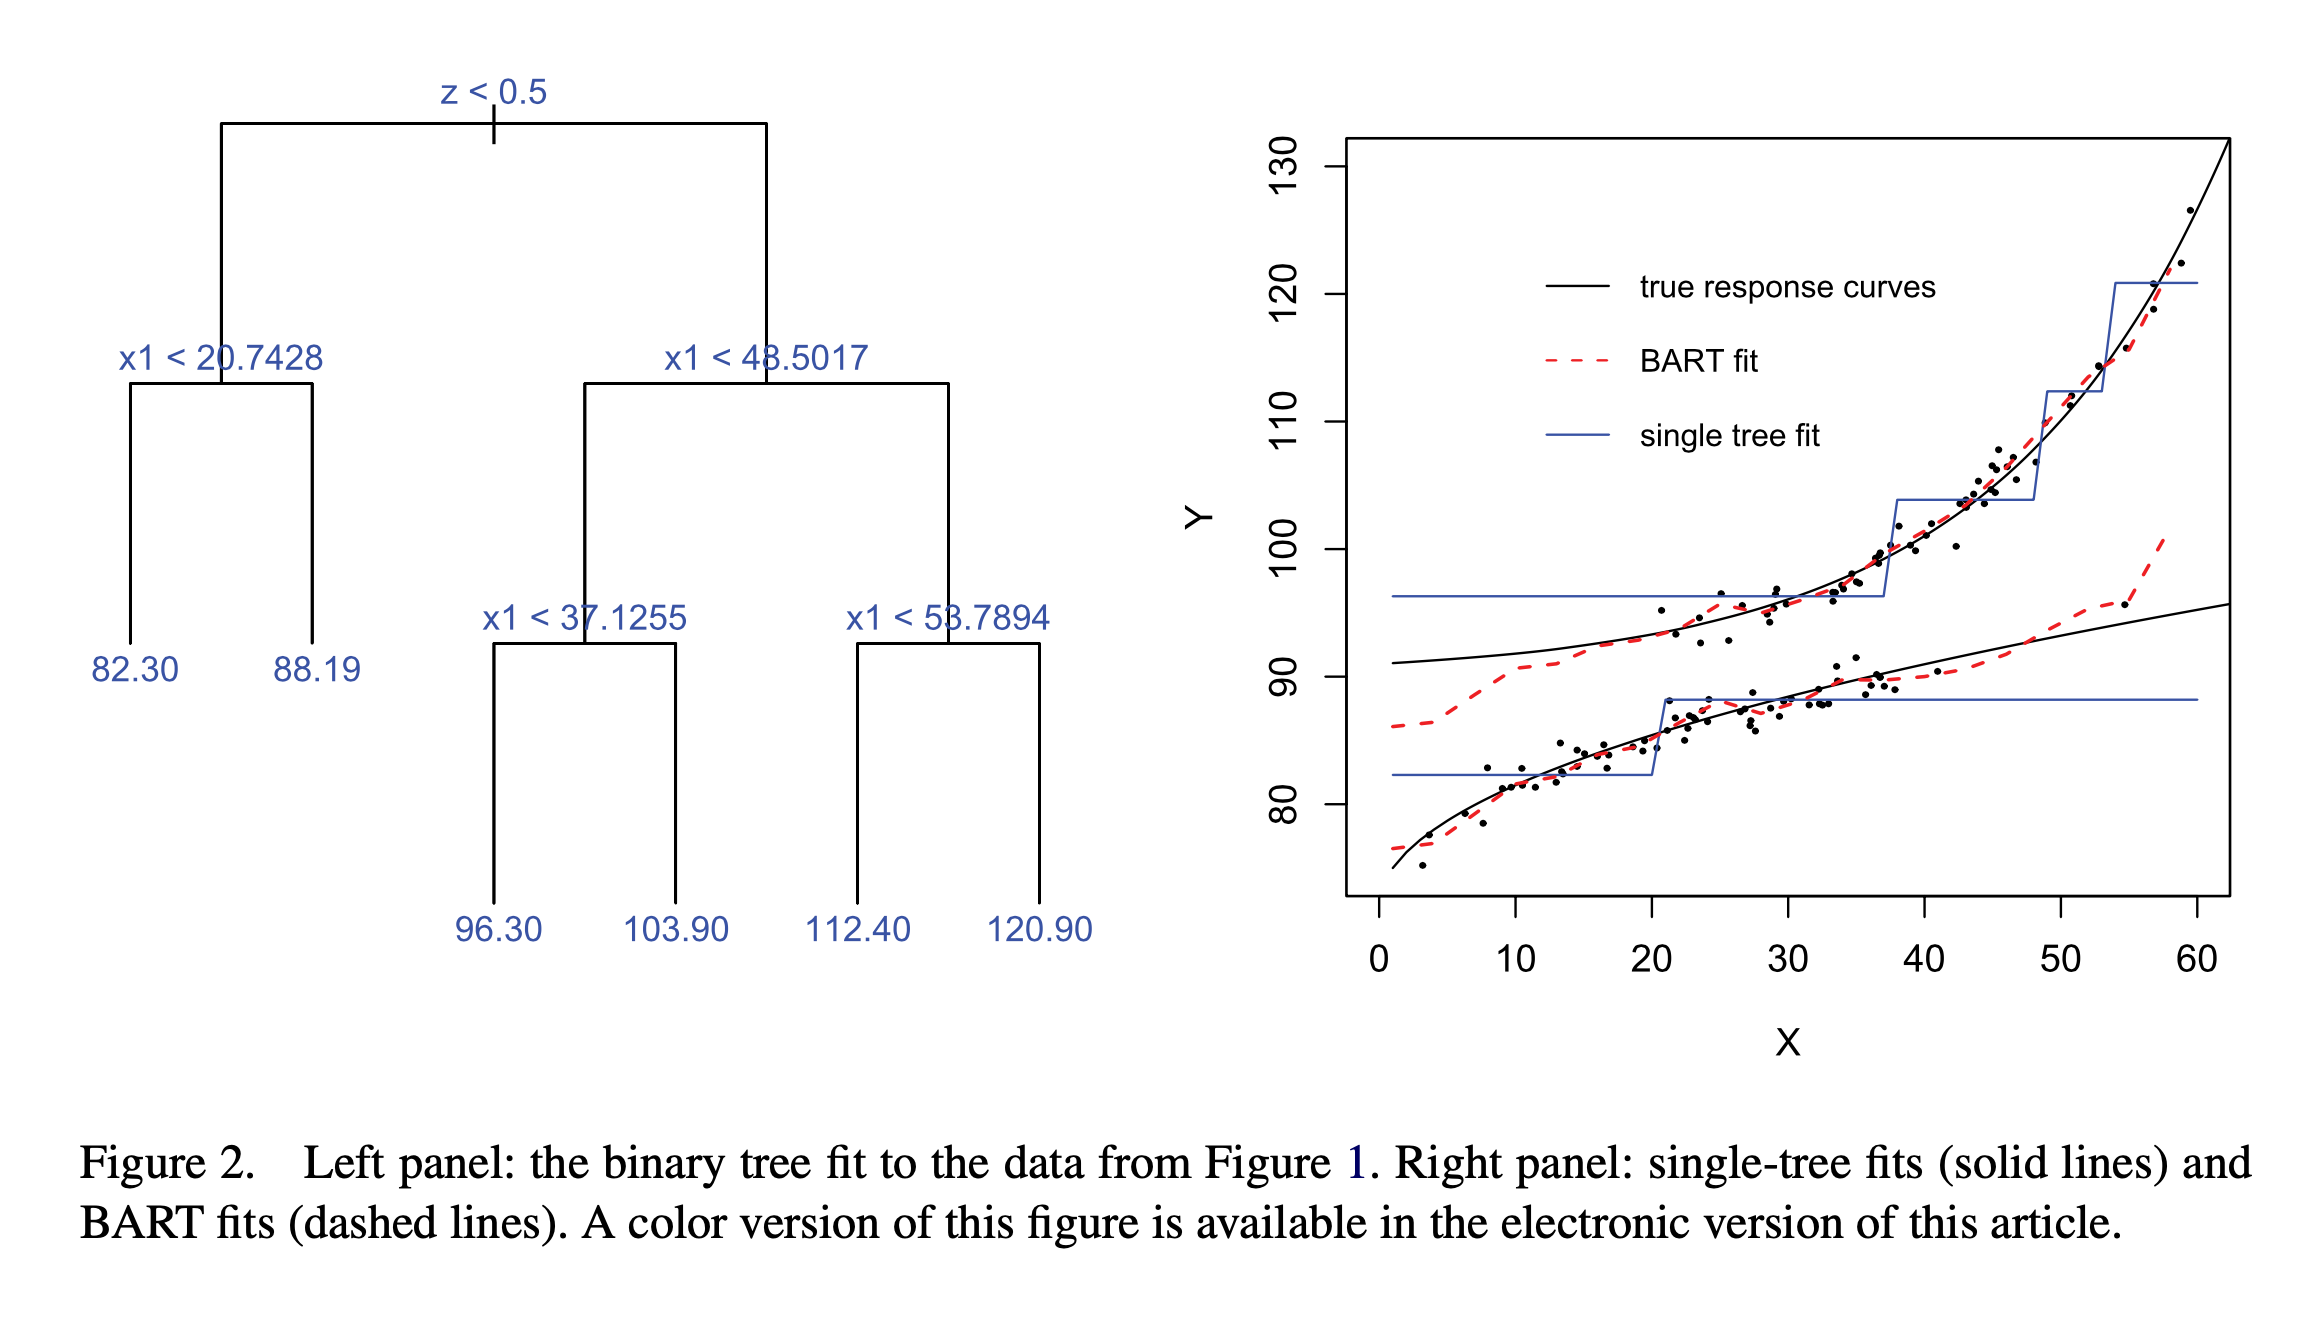
\includegraphics[height = 1.4in, trim = {0 2.5in 8in 0}, clip]{figures/hill2011_fig2} {\footnotesize (tree visualization from Hill 2011)}
\item Good at learning interactions among covariates
\item Ranger is fast
\end{itemize}
\end{frame}

\begin{frame}{A few algorithms you might consider: \texttt{BART}\footnote{Chipman, Hugh A., Edward I. George, and Robert E. McCulloch. ``\bref{https://projecteuclid.org/journals/annals-of-applied-statistics/volume-4/issue-1/BART-Bayesian-additive-regression-trees/10.1214/09-AOAS285.full}{BART: Bayesian additive regression trees.}" The Annals of Applied Statistics 4.1 (2010): 266-298.}}
\begin{itemize}
\item Bayesian version of random forest
\begin{itemize}
\item A prior regularizes estimates
\item Bonus: Free posterior variance estimates!
\end{itemize}
\item Warning: A bit slower than ranger
\end{itemize}
\end{frame}

\begin{frame}{A few algorithms you might consider: \texttt{SuperLearner}\footnote{Original: Van der Laan, M. J., Polley, E. C., \& Hubbard, A. E. (2007). \bref{https://www.degruyter.com/document/doi/10.2202/1544-6115.1309/html}{Super learner.} Statistical Applications in Genetics and Molecular Biology, 6(1).\\Good intro paper: Naimi, A. I., \& Balzer, L. B. (2018). \bref{https://link.springer.com/article/10.1007/s10654-018-0390-z}{Stacked generalization: an introduction to super learning.} European Journal of Epidemiology, 33(5), 459-464.}}
Why pick just one algorithm?
\begin{enumerate}
\item Fit many candidate learners $f_1(),f_2(),\dots$
\item Predict out-of-sample (using cross-validation)
\item Learn a set of weights to take a weighted average
$$\hat{f}(\vec\ell,a) = \hat\beta_1\underbrace{\hat{f}_1(\vec\ell,a)}_\text{e.g.~OLS} + \beta_2\underbrace{\hat{f}_2(\vec\ell,a)}_\text{e.g.~glmnet} + \beta_3\underbrace{\hat{f}_3(\vec\ell,a)}_\text{e.g.~ranger}$$
\end{enumerate}
\end{frame}

\begin{frame}{A few algorithms you might consider}

\begin{itemize}
\item You could use any of these
\item You could use something else
\item You could do the entire exercise with OLS
\begin{itemize}
\item try various functional forms
\end{itemize}
\item Choice is yours!
\end{itemize}

\end{frame}

\begin{frame}{How do I choose the black-box algorithm?\footnote{One can improve on this metric; we will come back to this later in the semester. See Van der Laan, M. J., \& Rose, S. (2018). \bref{https://link.springer.com/content/pdf/10.1007/978-3-319-65304-4.pdf}{Targeted learning in data science.} Springer International Publishing.}}
Could choose by an empirical metric of \bblue{predictive performance} \vskip .2in
\begin{tabular}{rl}
Task: & Predict $Y$ given $\{A,\vec{L}\}$\\
\\
Performance metric: & Minimize out-of-sample\\&mean squared error (MSE)
\end{tabular} \vskip .1in
Why MSE?
\begin{itemize}
\item The lowest-MSE predictor would be the true mean $\E(Y\mid \vec{L},A)$
\item Therefore, MSE is a principled metric when selecting an approximation
\end{itemize}
\end{frame}

\begin{frame}{Selecting an algorithm: The role of a train-test split}

\begin{tikzpicture}[y = .2in]
\node[anchor = north west] at (-3,2.5) {};
\node at (7,-11.5) {};
\node<2>[anchor = north west] at (-3,2.5) {1) Randomly assign cases to a \texttt{train} and \texttt{test} set};
\node<3-4>[anchor = north west] at (-3,2.5) {2) First, use only the \texttt{train} set.\only<4>{ Learn a prediction function.}};
\node<4>[anchor = south] at (4,0) {$f():\{\vec{L},A\}\rightarrow Y$};
\node<5-8>[anchor = north west] at (-3,2.5) {3) Open the \texttt{test} set.\only<6-8>{ Predict.}\only<7-8>{ Evaluate squared error.}\only<8>{ Average.}};
% Train set is 1, 2, 4, 8, 9
% Test set is 3, 5, 6, 7
\foreach \i in {1, 2, 4, 8, 9} {
	\only<1-4>{
	\node[font = \footnotesize] at (0,-\i) {Case \i};
	\node[font = \footnotesize] at (2,-\i) {$\{\vec{L}_\i,A_\i\}$};
	\node[font = \footnotesize] at (6.5,-\i) {$Y_\i$};
	\node<2->[font = \footnotesize] at (-2,-\i) {\texttt{train}};
	\draw<4->[->, thick] (3,-\i) -- (5,-\i);
	}
	\only<5->{
	\node[lightgray,font = \footnotesize] at (0,-\i) {Case \i};
	\node[lightgray,font = \footnotesize] at (2,-\i) {$\{\vec{L}_\i,A_\i\}$};
	\node[lightgray,font = \footnotesize] at (6.5,-\i) {$Y_\i$};
	\node<2->[lightgray,font = \footnotesize] at (-2,-\i) {\texttt{train}};
	\draw<4->[->, lightgray, thick] (3,-\i) -- (5,-\i);
	}
}
\foreach \i in {3, 5, 6, 7} {
	\only<1-2,5->{
	\node[font = \footnotesize] at (0,-\i) {Case \i};
	\node[font = \footnotesize] at (2,-\i) {$\{\vec{L}_\i,A_\i\}$};
	\node[font = \footnotesize] at (6.5,-\i) {$Y_\i$};
	\node<2->[font = \footnotesize] at (-2,-\i) {\texttt{test}};
	\draw<6->[->, thick] (3,-\i) -- (5,-\i);
	\node<6->[font = \footnotesize] at (5.5,-\i + .1) {$\hat{Y}_\i$};
	\node<7->[font = \footnotesize] at (5.2,-\i) {$($};
	\node<7->[font = \footnotesize] at (6,-\i) {${}-{}$};
	\node<7->[font = \footnotesize] at (6.8,-\i) {$)^2$};
	}
	\only<3-4>{
	\node[lightgray, font = \footnotesize] at (0,-\i) {Case \i};
	\node[lightgray, font = \footnotesize] at (2,-\i) {$\{\vec{L}_\i,A_\i\}$};
	\node[lightgray, font = \footnotesize] at (6.5,-\i) {$Y_\i$};
	\node<2->[lightgray, font = \footnotesize] at (-2,-\i) {\texttt{test}};
	}
}
	\node<8>[font = \footnotesize] at (3.5,-11) {$\widehat{\text{MSE}} = \frac{1}{n_{\texttt{test}}}\sum_{i\in\texttt{test}}$};
	\node<8>[font = \footnotesize] at (5.5,-11 + .1) {$\hat{Y}_i$};
	\node<8>[font = \footnotesize] at (6.5,-11) {$Y_i$};
	\node<8>[font = \footnotesize] at (5.2,-11) {$($};
	\node<8>[font = \footnotesize] at (6,-11) {${}-{}$};
	\node<8>[font = \footnotesize] at (6.8,-11) {$)^2$};
\end{tikzpicture}

\end{frame}


\begin{frame}{Is your SATT where it's at? \bgray{Data structure}}
\begin{itemize}
\item Simplified dataset on the course site: \bref{https://github.com/ilundberg/teaching/tree/master/info\_6751\_causal/data/lecture\_10.csv}{\texttt{lecture\_10.csv}}
\item This is one simulation from the many in Dorie et al.
\item Variables include
\begin{itemize}
\item \texttt{y}: outcome (numeric)
\item \texttt{z}: treatment (binary)
\item \texttt{x\_*}: confounders
\item \texttt{set}: I created this, coded \texttt{train} or \texttt{test}
\end{itemize}
\end{itemize} \vskip .2in
Code in \bref{https://github.com/ilundberg/teaching/tree/master/info\_6751\_causal/code\_examples/lecture\_10\_example\_code.R}{\texttt{lecture\_10\_example\_code.R}} can help you get started. \vskip .1in
At the end of class, you will produce on $\widehat{\text{SATT}}$. \\
Report your estimate here: \bref{https://tinyurl.com/SATTEstimate}{tinyurl.com/SATTEstimate}\\
I have the truth. We will see who is closest!

\end{frame}

\goalsframe

\begin{frame}{Let me know what you are thinking}

\begin{huge} \bref{https://tinyurl.com/CausalQuestions}{tinyurl.com/CausalQuestions} \end{huge}
\vskip .7in

Office hours TTh 11am-12pm and at \bref{https://calendly.com/ianlundberg/office-hours}{calendly.com/ianlundberg/office-hours}\\Come say hi!

\end{frame}

\end{document}

